%%%%%%%%%%%%%%%%%%%%%%%%%%%%%%%%%%%%%%%%%
% Short Sectioned Assignment
% LaTeX Template
% Version 1.0 (5/5/12)
%
% This template has been downloaded from:
% http://www.LaTeXTemplates.com
%
% Original author:
% Frits Wenneker (http://www.howtotex.com)
%
% License:
% CC BY-NC-SA 3.0 (http://creativecommons.org/licenses/by-nc-sa/3.0/)
%
%%%%%%%%%%%%%%%%%%%%%%%%%%%%%%%%%%%%%%%%%

%----------------------------------------------------------------------------------------
%	PACKAGES AND OTHER DOCUMENT CONFIGURATIONS
%----------------------------------------------------------------------------------------

\documentclass[paper=a4, fontsize=11pt]{scrartcl} % A4 paper and 11pt font size

\usepackage[T1]{fontenc} % Use 8-bit encoding that has 256 glyphs
\usepackage{fourier} % Use the Adobe Utopia font for the document - comment this line to return to the LaTeX default
\usepackage[english]{babel} % English language/hyphenation
\usepackage{amsmath,amsfonts,amsthm} % Math packages

\usepackage{graphicx}

\usepackage{sectsty} % Allows customizing section commands
\allsectionsfont{\centering \normalfont\scshape} % Make all sections centered, the default font and small caps

\usepackage{fancyhdr} % Custom headers and footers
\pagestyle{fancyplain} % Makes all pages in the document conform to the custom headers and footers
\fancyhead{} % No page header - if you want one, create it in the same way as the footers below
\fancyfoot[L]{} % Empty left footer
\fancyfoot[C]{} % Empty center footer
\fancyfoot[R]{\thepage} % Page numbering for right footer
\renewcommand{\headrulewidth}{0pt} % Remove header underlines
\renewcommand{\footrulewidth}{0pt} % Remove footer underlines
\setlength{\headheight}{13.6pt} % Customize the height of the header

\numberwithin{equation}{section} % Number equations within sections (i.e. 1.1, 1.2, 2.1, 2.2 instead of 1, 2, 3, 4)
\numberwithin{figure}{section} % Number figures within sections (i.e. 1.1, 1.2, 2.1, 2.2 instead of 1, 2, 3, 4)
\numberwithin{table}{section} % Number tables within sections (i.e. 1.1, 1.2, 2.1, 2.2 instead of 1, 2, 3, 4)

\setlength\parindent{0pt} % Removes all indentation from paragraphs - comment this line for an assignment with lots of text

%----------------------------------------------------------------------------------------
%	TITLE SECTION
%----------------------------------------------------------------------------------------

\newcommand{\horrule}[1]{\rule{\linewidth}{#1}} % Create horizontal rule command with 1 argument of height

\title{	
\normalfont \normalsize 
\textsc{BRSU} \\ [25pt] % Your university, school and/or department name(s)
\horrule{0.5pt} \\[0.4cm] % Thin top horizontal rule
\huge Neural Networks\\Assignment 2 \\ % The assignment title
\horrule{2pt} \\[0.5cm] % Thick bottom horizontal rule
}

\author{Bastian Lang} % Your name

\date{\normalsize\today} % Today's date or a custom date

\begin{document}

\maketitle % Print the title

\section{Read chapter 2 from Haykin's book until 2.13 (leaving out Statistical learning theory to
end of chapter) and summarize or sketch your insights in mind-map or an outline or a
summary.}

See figure \ref{fig1}.

\begin{figure}[ht]
	\centering
  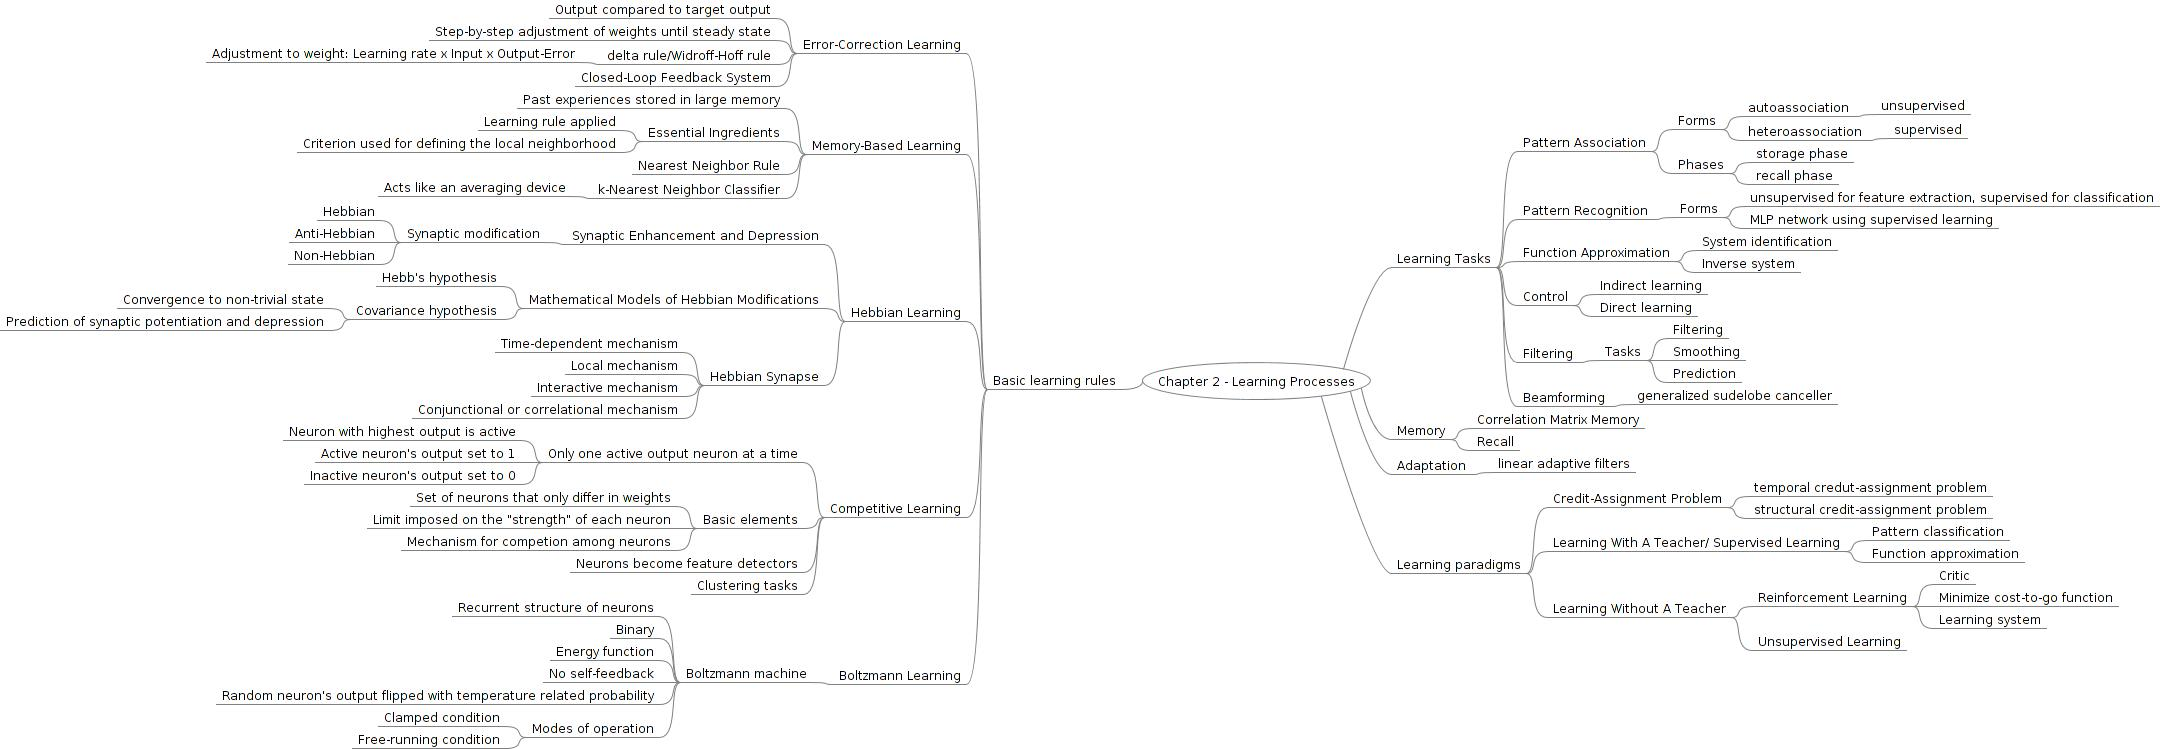
\includegraphics[width=1\textheight, angle=90]{mindmap.jpeg}
	\caption{Mindmap}
	\label{fig1}
\end{figure}

\section{Design a perceptron that computes the following Boolean function:}

\subsection{$f(x_1 , x_2 ) = NOT(x_1 AND x_2 )$}

A single layer perceptron displays a simple linar function. For this problem it looks like:\\
$STEP(w_1x_1 + w_2x_2 + w_0) = y$\\
For the given functions the following equations have to hold true:\\
$w_1 + w_2 < -w_0$\\
$w_1 > -w_0$\\
$w_2 > -w_0$\\
$0 > -w_0$\\\\

This is true for $w_0 = 0.2, w_1 = w_2 = -0.15$\\
(See figure \ref{figNotAnd})

\begin{figure}[ht]
	\centering
  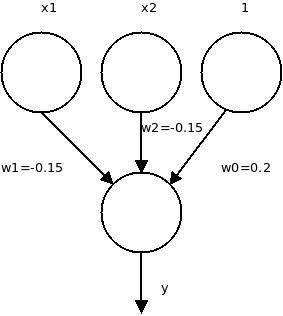
\includegraphics[width=0.5\textheight]{NotAnd.jpeg}
	\caption{NotAnd}
	\label{figNotAnd}
\end{figure}

\subsection{$f(x_1 , x_2 , x_3 ) = (x_1 AND x_2 ) OR x_3$}

The SLP function does look like:\\
$STEP(w_1x_1 + w_2x_2 + w_3x_3 + w_0) = y$\\\\
The following equations have to hold true:\\
$w_1 + w_2 + w_3 > -w_0$\\
$w_2 + w_3 > -w_0$\\
$w_1 + w_3 > -w_0$\\
$w_3 > -w_0$\\
$w_1 + w_2 > -w_0$\\
$w_1 < -w_0$\\
$w_2 < -w_0$\\\\

This is true for $w_0 = -0.2, w_1 = w_2 = 0.15, w_3 = 0.3$\\
(See figure \ref{figAndOr})

\begin{figure}[ht]
	\centering
  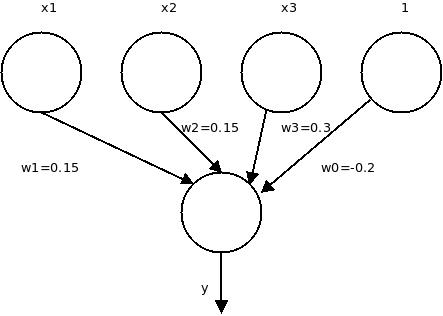
\includegraphics[width=0.5\textheight]{AndOr.jpeg}
	\caption{AndOr}
	\label{figAndOr}
\end{figure}

\section{}

\subsection{A basic limitation of the perceptron is that it cannot implement the EXCLUSIVE OR
function. Explain the reason for this limitation.}

For XOR, the following equations have to be true:\\
$w_1 + w_2 < -w_0$\\
$0 < -w_0$\\
$w_1 > -w_0$\\
$w_2 > -w_0$\\\\

From these equations:\\
$w_0 > 0 \rightarrow w_1 > 0 \land w_2 > 0$\\
$w_1 + w_2 < -w_0 < w_1 \land w_1 + w_2 < -w_0 < w_2$\\
$\rightarrow w_1 < 0 \land w_2 < 0$\\\\

This contradiction shows that XOR is not solvable using a Single Layer Perceptron.

\subsection{Show that neural networks with one hidden layer can describe all Boolean functions.}

Every boolean function can be written in KNF, i.e. a conjunction of disjunctions.\\
The connection from the input layer to the hidden layer can be seen as n SLPs, where n is the number of neurons in the hidden layer. So it would be possible to let each of those SLPs represent one disjunction.\\
The connection from the hidden layer to the single output neuron can again be seen as a single SLP.\\
This SLP is able to represent the conjunction of all former disjunctions.\\
Thus a network with one hidden layer is able to describe any boolean function because any boolean function can be written as a conjunction of disjunctions.


\end{document}